\documentclass[margin=5mm, tikz]{standalone}
\usepackage[utf8x]{inputenc}
\usepackage{tikz}
\usepackage{siunitx}
\begin{document}
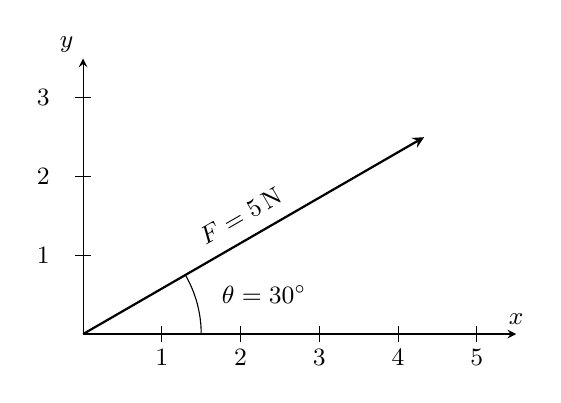
\begin{tikzpicture}
    
    \draw [-stealth] (0, 0) -- (5.5, 0) node [above, pos=1] {\small{$x$}};
    \draw [-stealth] (0, 0) -- (0, 3.5) node [left, pos=1.05] {\small{$y$}};

    \foreach \y in {1, 2, 3}
        { \draw (-0.3, \y) node [left] {\small{$\y$}};
          \draw (-0.1, \y) -- (0.1, \y);}
    
    \foreach \x in {1, 2, 3, 4, 5}
        { \draw (\x, -0.3) node {\small{$\x$}};
        \draw (\x, -0.1) -- (\x, 0.1);}

    \draw [-stealth, thick] (0, 0) -- (4.33, 2.5);

    \node at (2, 1.5) [rotate=30] {\small$F = \SI{5}{\newton}$};

    \draw (1.5, 0) arc(0:30:1.5);
    \node at (2.3, 0.5) {\small{$\theta = \ang{30}$}};
    
    
\end{tikzpicture}
\end{document}